\clearpage


\section{بناء الخوارزمية البرمجية \textenglish{(Ladder Logic Implementation)}}
\label{sec:ladder_code}

يُمثل المخطط السلمي \textenglish{(Ladder Diagram)} العقل المدبر للمنظومة، حيث تمت كتابة الخوارزمية باستخدام بيئة التطوير \textenglish{WPLSoft}. تم تصميم الكود ليتعامل مع متغيرات ديناميكية سريعة جداً، مما استدعى استخدام تعليمات متقدمة بحجم 32-بت \textenglish{(Double Word)} لضمان عدم حدوث أي تجاوز لسعة المسجلات \textenglish{(Overflow)} أثناء قراءة المشفر أو إرسال النبضات.

الشكل (\ref{fig:ladder_code}) يوضح المخطط السلمي الكامل للمنظومة كما تم تصديره من بيئة التطوير.


\subsection{التحليل الهندسي لبنية الكود}
ينقسم الكود البرمجي إلى أربع كتل وظيفية رئيسية، تم تصميم كل منها لمعالجة تحدٍ ديناميكي محدد في الآلة:

\subsubsection{1. العداد السريع والتصفير الذاتي \textenglish{(High-Speed Counter \& Self-Reset)}}
تم استخدام التعليمة \LR{DCNT C254 K0} لتفعيل قراءة نبضات المشفر القائد. القيمة \LR{K0} هنا مقصودة هندسياً؛ حيث تُوجه المتحكم لتجاهل أي هدف للعداد وجعله يعمل كـ "مسجل موقع مستمر". 
ولضمان عدم تراكم الخطأ أو ضياع مسافة أثناء عملية القص، تم ابتكار حيلة "التصفير الذاتي". بدلاً من انتظار انتهاء دورة القص لتصفير العداد، يتم أخذ نبضة حافة صاعدة \textenglish{(Rising Edge)} من ماركر المزامنة \LR{M2} لتصفير العداد \LR{C254} في اللحظة الأولى لبدء القطع، مما يضمن دقة متناهية للقطعة التالية حتى وإن كان المنتج مستمراً بالحركة.

\subsubsection{2. اتخاذ قرار القص \textenglish{(Cutting Decision)}}
نظراً لأن العداد \LR{C254} هو مسجل 32-بت، تم استخدام تعليمة المقارنة المزدوجة \LR{DLD>= C254 K2000}. هذا السطر يراقب القيمة المتراكمة باستمرار، وبمجرد وصولها إلى 2000 (والتي تكافئ طول الصابون المطلوب 20 سم)، يتم تفعيل حالة الانطلاق والمزامنة \LR{M2} بشكل فوري.

\subsubsection{3. توليد النبضات والتزامن \textenglish{(Pulse Output \& Synchronization)}}
لتحقيق التطابق الحركي مع السير الناقل، تم إرسال نبضات عالية التردد لدرايف السيرفو باستخدام التعليمة \LR{DPLSY K150000 K0 Y0}. 
التردد 150,000 هرتز تم حسابه بدقة بناءً على سرعة المنتج (150مم/ثانية) والنسبة الإلكترونية المعدلة في السيرفو (500 نبضة/مم). أما القيمة \LR{K0} في المسافة، فتعني إبقاء توليد النبضات مستمراً لضمان بقاء المقص متزامناً تماماً مع المنتج طوال فترة نزول الشفرة، على أن يتم الإيقاف لاحقاً عبر المؤقتات الزمنية.

\subsubsection{4. شبكات الحماية الميكانيكية \textenglish{(Protection Networks)}}
تم وضع تماسات حساسات نهاية الشوط \LR{X7} و \LR{X10} في نهاية الكود كشبكات حماية مستقلة. في حال تجاوز العربة لمسارها المسموح، تقوم هذه التماسات بعمل \textenglish{Reset} لحالات الحركة (\LR{M1, M2, M3}) مما يقطع النبضات عن التعليمة \LR{DPLSY} فوراً. هذه الطريقة البرمجية توقف الحركة مع إبقاء المحرك ممغنطاً \textenglish{(Servo Hold)} لمنع اندفاع العربة بسبب القصور الذاتي، وهو إجراء أأمن بكثير من قطع إشارة التفعيل \LR{Y2} بشكل مباشر.

\begin{figure}[h!]
    \centering
    % تأكد من أن مسار المجلد resources صحيح ومطابق لما لديك في المشروع
    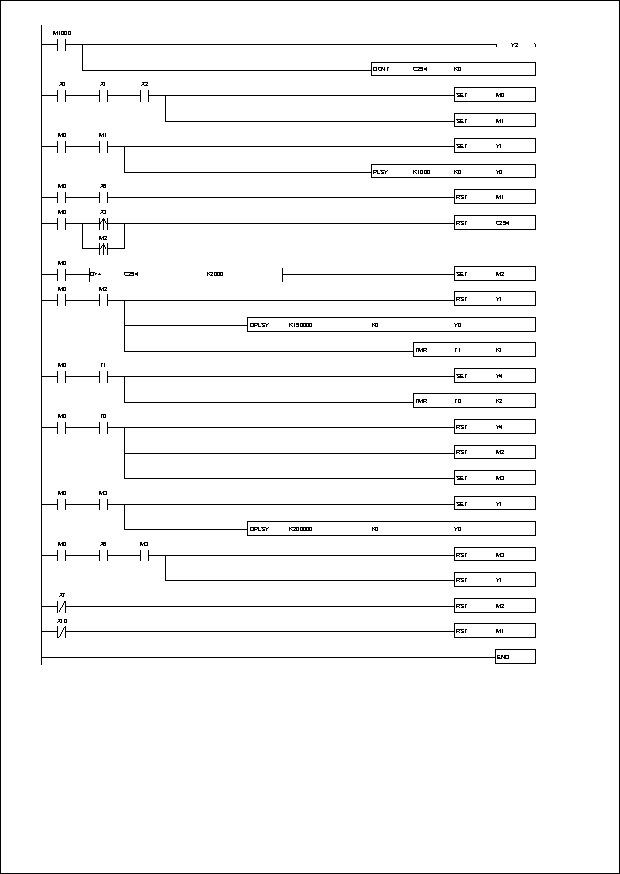
\includegraphics[width=\textwidth]{resources/code/flying_shear_code.pdf} 
    \caption[المخطط السلمي لخوارزمية المقص الطائر]{\centering المخطط السلمي لخوارزمية المقص الطائر، يوضح شبكات المزامنة، العدادات السريعة، وحماية نهايات الشوط.}
    \label{fig:ladder_code}
\end{figure}
